% Options for packages loaded elsewhere
% Options for packages loaded elsewhere
\PassOptionsToPackage{unicode}{hyperref}
\PassOptionsToPackage{hyphens}{url}
\PassOptionsToPackage{dvipsnames,svgnames,x11names}{xcolor}
%
\documentclass[
  letterpaper,
  DIV=11,
  numbers=noendperiod]{scrartcl}
\usepackage{xcolor}
\usepackage{amsmath,amssymb}
\setcounter{secnumdepth}{-\maxdimen} % remove section numbering
\usepackage{iftex}
\ifPDFTeX
  \usepackage[T1]{fontenc}
  \usepackage[utf8]{inputenc}
  \usepackage{textcomp} % provide euro and other symbols
\else % if luatex or xetex
  \usepackage{unicode-math} % this also loads fontspec
  \defaultfontfeatures{Scale=MatchLowercase}
  \defaultfontfeatures[\rmfamily]{Ligatures=TeX,Scale=1}
\fi
\usepackage{lmodern}
\ifPDFTeX\else
  % xetex/luatex font selection
\fi
% Use upquote if available, for straight quotes in verbatim environments
\IfFileExists{upquote.sty}{\usepackage{upquote}}{}
\IfFileExists{microtype.sty}{% use microtype if available
  \usepackage[]{microtype}
  \UseMicrotypeSet[protrusion]{basicmath} % disable protrusion for tt fonts
}{}
\makeatletter
\@ifundefined{KOMAClassName}{% if non-KOMA class
  \IfFileExists{parskip.sty}{%
    \usepackage{parskip}
  }{% else
    \setlength{\parindent}{0pt}
    \setlength{\parskip}{6pt plus 2pt minus 1pt}}
}{% if KOMA class
  \KOMAoptions{parskip=half}}
\makeatother
% Make \paragraph and \subparagraph free-standing
\makeatletter
\ifx\paragraph\undefined\else
  \let\oldparagraph\paragraph
  \renewcommand{\paragraph}{
    \@ifstar
      \xxxParagraphStar
      \xxxParagraphNoStar
  }
  \newcommand{\xxxParagraphStar}[1]{\oldparagraph*{#1}\mbox{}}
  \newcommand{\xxxParagraphNoStar}[1]{\oldparagraph{#1}\mbox{}}
\fi
\ifx\subparagraph\undefined\else
  \let\oldsubparagraph\subparagraph
  \renewcommand{\subparagraph}{
    \@ifstar
      \xxxSubParagraphStar
      \xxxSubParagraphNoStar
  }
  \newcommand{\xxxSubParagraphStar}[1]{\oldsubparagraph*{#1}\mbox{}}
  \newcommand{\xxxSubParagraphNoStar}[1]{\oldsubparagraph{#1}\mbox{}}
\fi
\makeatother

\usepackage{color}
\usepackage{fancyvrb}
\newcommand{\VerbBar}{|}
\newcommand{\VERB}{\Verb[commandchars=\\\{\}]}
\DefineVerbatimEnvironment{Highlighting}{Verbatim}{commandchars=\\\{\}}
% Add ',fontsize=\small' for more characters per line
\usepackage{framed}
\definecolor{shadecolor}{RGB}{241,243,245}
\newenvironment{Shaded}{\begin{snugshade}}{\end{snugshade}}
\newcommand{\AlertTok}[1]{\textcolor[rgb]{0.68,0.00,0.00}{#1}}
\newcommand{\AnnotationTok}[1]{\textcolor[rgb]{0.37,0.37,0.37}{#1}}
\newcommand{\AttributeTok}[1]{\textcolor[rgb]{0.40,0.45,0.13}{#1}}
\newcommand{\BaseNTok}[1]{\textcolor[rgb]{0.68,0.00,0.00}{#1}}
\newcommand{\BuiltInTok}[1]{\textcolor[rgb]{0.00,0.23,0.31}{#1}}
\newcommand{\CharTok}[1]{\textcolor[rgb]{0.13,0.47,0.30}{#1}}
\newcommand{\CommentTok}[1]{\textcolor[rgb]{0.37,0.37,0.37}{#1}}
\newcommand{\CommentVarTok}[1]{\textcolor[rgb]{0.37,0.37,0.37}{\textit{#1}}}
\newcommand{\ConstantTok}[1]{\textcolor[rgb]{0.56,0.35,0.01}{#1}}
\newcommand{\ControlFlowTok}[1]{\textcolor[rgb]{0.00,0.23,0.31}{\textbf{#1}}}
\newcommand{\DataTypeTok}[1]{\textcolor[rgb]{0.68,0.00,0.00}{#1}}
\newcommand{\DecValTok}[1]{\textcolor[rgb]{0.68,0.00,0.00}{#1}}
\newcommand{\DocumentationTok}[1]{\textcolor[rgb]{0.37,0.37,0.37}{\textit{#1}}}
\newcommand{\ErrorTok}[1]{\textcolor[rgb]{0.68,0.00,0.00}{#1}}
\newcommand{\ExtensionTok}[1]{\textcolor[rgb]{0.00,0.23,0.31}{#1}}
\newcommand{\FloatTok}[1]{\textcolor[rgb]{0.68,0.00,0.00}{#1}}
\newcommand{\FunctionTok}[1]{\textcolor[rgb]{0.28,0.35,0.67}{#1}}
\newcommand{\ImportTok}[1]{\textcolor[rgb]{0.00,0.46,0.62}{#1}}
\newcommand{\InformationTok}[1]{\textcolor[rgb]{0.37,0.37,0.37}{#1}}
\newcommand{\KeywordTok}[1]{\textcolor[rgb]{0.00,0.23,0.31}{\textbf{#1}}}
\newcommand{\NormalTok}[1]{\textcolor[rgb]{0.00,0.23,0.31}{#1}}
\newcommand{\OperatorTok}[1]{\textcolor[rgb]{0.37,0.37,0.37}{#1}}
\newcommand{\OtherTok}[1]{\textcolor[rgb]{0.00,0.23,0.31}{#1}}
\newcommand{\PreprocessorTok}[1]{\textcolor[rgb]{0.68,0.00,0.00}{#1}}
\newcommand{\RegionMarkerTok}[1]{\textcolor[rgb]{0.00,0.23,0.31}{#1}}
\newcommand{\SpecialCharTok}[1]{\textcolor[rgb]{0.37,0.37,0.37}{#1}}
\newcommand{\SpecialStringTok}[1]{\textcolor[rgb]{0.13,0.47,0.30}{#1}}
\newcommand{\StringTok}[1]{\textcolor[rgb]{0.13,0.47,0.30}{#1}}
\newcommand{\VariableTok}[1]{\textcolor[rgb]{0.07,0.07,0.07}{#1}}
\newcommand{\VerbatimStringTok}[1]{\textcolor[rgb]{0.13,0.47,0.30}{#1}}
\newcommand{\WarningTok}[1]{\textcolor[rgb]{0.37,0.37,0.37}{\textit{#1}}}

\usepackage{longtable,booktabs,array}
\usepackage{calc} % for calculating minipage widths
% Correct order of tables after \paragraph or \subparagraph
\usepackage{etoolbox}
\makeatletter
\patchcmd\longtable{\par}{\if@noskipsec\mbox{}\fi\par}{}{}
\makeatother
% Allow footnotes in longtable head/foot
\IfFileExists{footnotehyper.sty}{\usepackage{footnotehyper}}{\usepackage{footnote}}
\makesavenoteenv{longtable}
\usepackage{graphicx}
\makeatletter
\newsavebox\pandoc@box
\newcommand*\pandocbounded[1]{% scales image to fit in text height/width
  \sbox\pandoc@box{#1}%
  \Gscale@div\@tempa{\textheight}{\dimexpr\ht\pandoc@box+\dp\pandoc@box\relax}%
  \Gscale@div\@tempb{\linewidth}{\wd\pandoc@box}%
  \ifdim\@tempb\p@<\@tempa\p@\let\@tempa\@tempb\fi% select the smaller of both
  \ifdim\@tempa\p@<\p@\scalebox{\@tempa}{\usebox\pandoc@box}%
  \else\usebox{\pandoc@box}%
  \fi%
}
% Set default figure placement to htbp
\def\fps@figure{htbp}
\makeatother





\setlength{\emergencystretch}{3em} % prevent overfull lines

\providecommand{\tightlist}{%
  \setlength{\itemsep}{0pt}\setlength{\parskip}{0pt}}



 


\KOMAoption{captions}{tableheading}
\makeatletter
\@ifpackageloaded{caption}{}{\usepackage{caption}}
\AtBeginDocument{%
\ifdefined\contentsname
  \renewcommand*\contentsname{Table of contents}
\else
  \newcommand\contentsname{Table of contents}
\fi
\ifdefined\listfigurename
  \renewcommand*\listfigurename{List of Figures}
\else
  \newcommand\listfigurename{List of Figures}
\fi
\ifdefined\listtablename
  \renewcommand*\listtablename{List of Tables}
\else
  \newcommand\listtablename{List of Tables}
\fi
\ifdefined\figurename
  \renewcommand*\figurename{Figure}
\else
  \newcommand\figurename{Figure}
\fi
\ifdefined\tablename
  \renewcommand*\tablename{Table}
\else
  \newcommand\tablename{Table}
\fi
}
\@ifpackageloaded{float}{}{\usepackage{float}}
\floatstyle{ruled}
\@ifundefined{c@chapter}{\newfloat{codelisting}{h}{lop}}{\newfloat{codelisting}{h}{lop}[chapter]}
\floatname{codelisting}{Listing}
\newcommand*\listoflistings{\listof{codelisting}{List of Listings}}
\makeatother
\makeatletter
\makeatother
\makeatletter
\@ifpackageloaded{caption}{}{\usepackage{caption}}
\@ifpackageloaded{subcaption}{}{\usepackage{subcaption}}
\makeatother
\usepackage{bookmark}
\IfFileExists{xurl.sty}{\usepackage{xurl}}{} % add URL line breaks if available
\urlstyle{same}
\hypersetup{
  pdftitle={EVALUACIÓN MIDTERM - Modelamiento de balance de masa},
  pdfauthor={Ruben Basantes},
  colorlinks=true,
  linkcolor={blue},
  filecolor={Maroon},
  citecolor={Blue},
  urlcolor={Blue},
  pdfcreator={LaTeX via pandoc}}


\title{EVALUACIÓN MIDTERM - Modelamiento de balance de masa}
\author{Ruben Basantes}
\date{2025-10-04}
\begin{document}
\maketitle


\subsection{¿Qué queremos modelar?}\label{quuxe9-queremos-modelar}

Vamos a modelar la variacion de elevacion sobre una superficie
terrestre. Este tipo de fenomenos ocurre debido a deformaciones
superficiales relacionadas al nivel freatico, morfologias promensas a
movimientos en masa, undimientos superficiales, entre otros aspectos
geologicos propios el sitio

\subsection{Hipotesis}\label{hipotesis}

Las deformaciones superficiales estan estrechamente relacionadas con
parametros geologicos y climaticos

\subsection{¿Qué es la regresión lineal
simple?}\label{quuxe9-es-la-regresiuxf3n-lineal-simple}

Es un método estadístico que se enfoca en analizar la relación lineal
entre dos variables:

\begin{itemize}
\tightlist
\item
  Una \textbf{variable independiente} X (Variacion de elevacion de la
  superficie con respecto al timpo dhdt)
\item
  Una \textbf{variable dependiente} Y (orientaciones de los flancos de
  las montanas `asp1', rugosidad del terreno `rgh1', morfologias
  topograficas `tpi1', precipitaciones `prec1')
\end{itemize}

Se uso una base de datos propia construida a partir de modelos digitales
de elevacion

El modelo tiene esta forma:

Y = b0 + b1*X

Donde:

\begin{itemize}
\tightlist
\item
  b0: es la \textbf{intersección (intercepto)}. Es el valor de Y cuando
  X = 0.\\
\item
  b1: es la \textbf{pendiente de la recta}, y representa cuánto cambia Y
  por cada unidad que aumenta X.
\end{itemize}

Queremos encontrar una recta que se ajuste lo mejor posible a nuestros
datos, es decir que exista una minima diferencia entre el valor real y
lo predicho. Este es el criterio de \textbf{mínimos cuadrados}.

\subsection{0. Importando librerias}\label{importando-librerias}

Se importan las librerias desde los paquetes

\begin{Shaded}
\begin{Highlighting}[]
\ImportTok{import}\NormalTok{ pandas }\ImportTok{as}\NormalTok{ pd}
\ImportTok{import}\NormalTok{ numpy }\ImportTok{as}\NormalTok{ np}
\ImportTok{import}\NormalTok{ geopandas }\ImportTok{as}\NormalTok{ gpd}
\ImportTok{import}\NormalTok{ matplotlib.pyplot }\ImportTok{as}\NormalTok{ plt}
\ImportTok{from}\NormalTok{ sklearn.model\_selection }\ImportTok{import}\NormalTok{ train\_test\_split}
\ImportTok{from}\NormalTok{ sklearn.preprocessing }\ImportTok{import}\NormalTok{ StandardScaler, PolynomialFeatures}
\ImportTok{from}\NormalTok{ sklearn.pipeline }\ImportTok{import}\NormalTok{ Pipeline}
\ImportTok{from}\NormalTok{ sklearn.linear\_model }\ImportTok{import}\NormalTok{ LinearRegression}
\ImportTok{from}\NormalTok{ sklearn.model\_selection }\ImportTok{import}\NormalTok{ learning\_curve}
\ImportTok{from}\NormalTok{ sklearn.metrics }\ImportTok{import}\NormalTok{ mean\_squared\_error, r2\_score}
\ImportTok{import}\NormalTok{ seaborn }\ImportTok{as}\NormalTok{ sns}
\end{Highlighting}
\end{Shaded}

\subsection{1. Carga y exploración inicial del
dataset.}\label{carga-y-exploraciuxf3n-inicial-del-dataset.}

Se cargan los datos del archivo .csv, que proviene de una cobertura de
puntos en formato shapefile.La tabla contiene atributos asociados a los
balanves de masa.

\begin{Shaded}
\begin{Highlighting}[]
\NormalTok{df }\OperatorTok{=}\NormalTok{ gpd.read\_file(}\StringTok{"ant\_20222016\_Dh\_adjslp\_pts.dbf"}\NormalTok{)}
\CommentTok{\# Ver primeras filas}
\NormalTok{df.head()}
\end{Highlighting}
\end{Shaded}

\begin{longtable}[]{@{}llllllllllllll@{}}
\toprule\noalign{}
& VALUE & Este & Norte & asp1 & rgh1 & slp1 & tpi1 & tri1 & elev1 &
prec1 & tmed1 & dhdt & geometry \\
\midrule\noalign{}
\endhead
\bottomrule\noalign{}
\endlastfoot
0 & 5.083925 & 816872.728 & 9947471.064 & 0.109970 & 1.692383 &
20.886478 & -0.075195 & 1.031517 & 4861.926758 & 1597.466675 & 4 &
0.847321 & None \\
1 & 4.190065 & 816876.728 & 9947471.064 & 350.337708 & 1.587891 &
20.204298 & -0.185059 & 0.905296 & 4861.905273 & 1597.466675 & 4 &
0.698344 & None \\
2 & 3.812052 & 816880.728 & 9947471.064 & 343.757568 & 1.791992 &
19.912228 & -0.005859 & 0.305124 & 4862.399414 & 1597.466675 & 4 &
0.635342 & None \\
3 & 3.402457 & 816884.728 & 9947471.064 & 335.548126 & 1.941406 &
20.086668 & -0.081055 & 0.596693 & 4862.826172 & 1597.466675 & 4 &
0.567076 & None \\
4 & 3.139728 & 816888.728 & 9947471.064 & 346.701843 & 1.399414 &
16.271687 & 0.032715 & 0.829091 & 4863.404297 & 1597.466675 & 4 &
0.523288 & None \\
\end{longtable}

Se identifican las variables con valores faltantes y se visualizan en un
gráfico de barras. sto permite decidir si imputar valores o eliminar
registros incompletos.

\begin{Shaded}
\begin{Highlighting}[]
\CommentTok{\# Porcentaje de valores faltantes por columna}
\NormalTok{nan\_percent }\OperatorTok{=}\NormalTok{ df.isna().mean() }\OperatorTok{*} \DecValTok{100}
\NormalTok{nan\_percent\_sorted }\OperatorTok{=}\NormalTok{ nan\_percent.sort\_values(ascending}\OperatorTok{=}\VariableTok{False}\NormalTok{).}\BuiltInTok{round}\NormalTok{(}\DecValTok{2}\NormalTok{)}

\BuiltInTok{print}\NormalTok{(}\StringTok{"Porcentaje de valores faltantes por columna:"}\NormalTok{)}
\BuiltInTok{print}\NormalTok{(nan\_percent\_sorted)}

\CommentTok{\# === Visualización opcional con gráfico de barras ===}
\NormalTok{nan\_percent\_sorted[nan\_percent\_sorted }\OperatorTok{\textgreater{}} \DecValTok{0}\NormalTok{].plot(}
\NormalTok{    kind}\OperatorTok{=}\StringTok{\textquotesingle{}barh\textquotesingle{}}\NormalTok{, color}\OperatorTok{=}\StringTok{\textquotesingle{}salmon\textquotesingle{}}\NormalTok{, figsize}\OperatorTok{=}\NormalTok{(}\DecValTok{8}\NormalTok{,}\DecValTok{5}\NormalTok{)}
\NormalTok{)}
\NormalTok{plt.title(}\StringTok{"Porcentaje de valores faltantes por variable"}\NormalTok{)}
\NormalTok{plt.xlabel(}\StringTok{"Porcentaje (\%)"}\NormalTok{)}
\NormalTok{plt.ylabel(}\StringTok{"Variable"}\NormalTok{)}
\NormalTok{plt.grid(axis}\OperatorTok{=}\StringTok{\textquotesingle{}x\textquotesingle{}}\NormalTok{, linestyle}\OperatorTok{=}\StringTok{\textquotesingle{}{-}{-}\textquotesingle{}}\NormalTok{, alpha}\OperatorTok{=}\FloatTok{0.7}\NormalTok{)}
\NormalTok{plt.show()}
\end{Highlighting}
\end{Shaded}

\begin{verbatim}
Porcentaje de valores faltantes por columna:
geometry    100.00
tri1          0.05
asp1          0.03
rgh1          0.03
slp1          0.03
tpi1          0.03
VALUE         0.00
Este          0.00
Norte         0.00
elev1         0.00
prec1         0.00
tmed1         0.00
dhdt          0.00
dtype: float64
\end{verbatim}

\pandocbounded{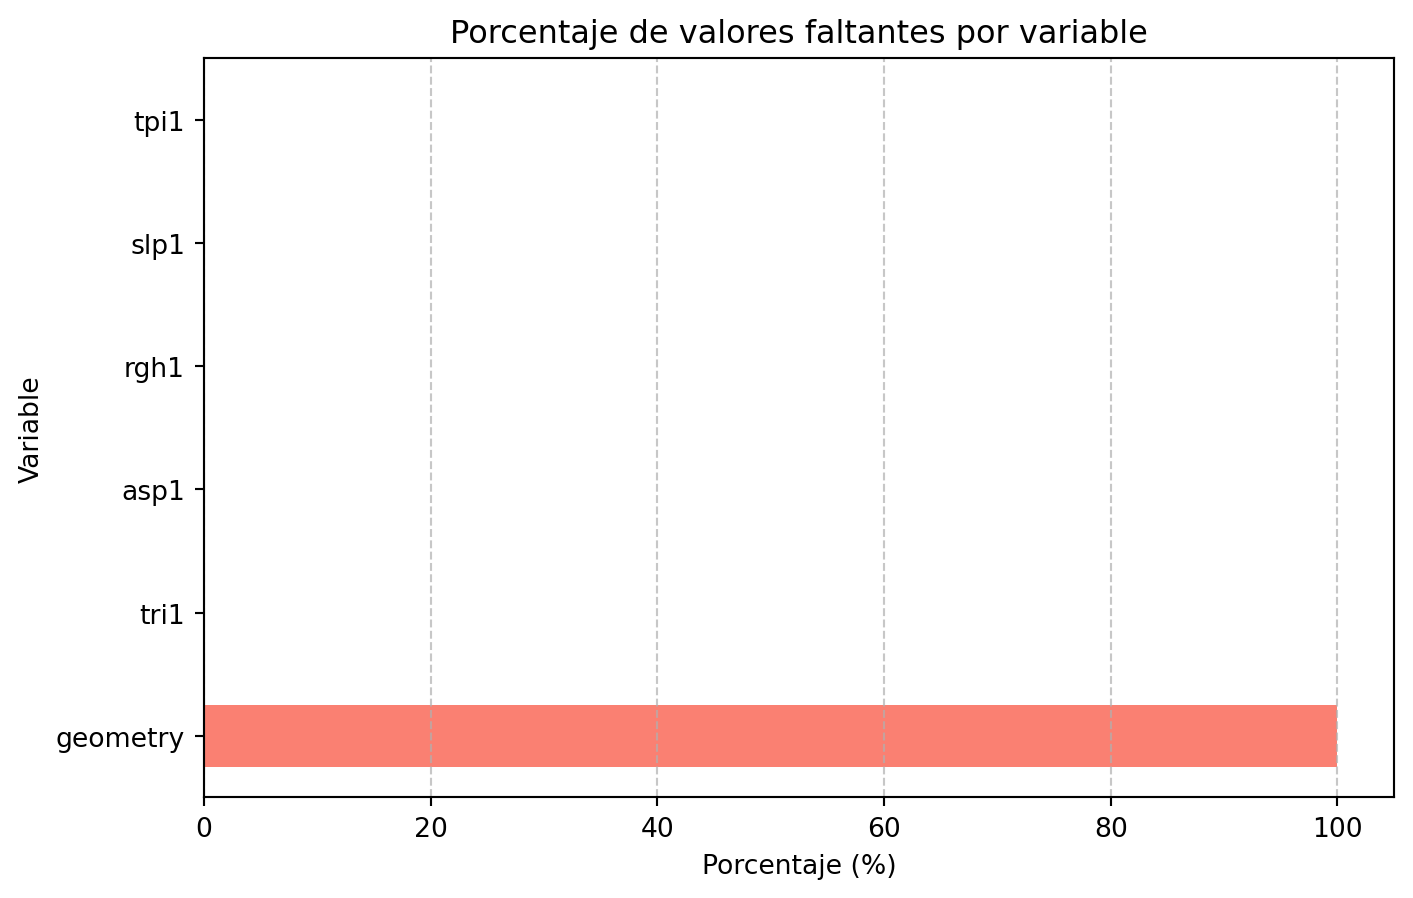
\includegraphics[keepaspectratio]{index_files/figure-pdf/cell-4-output-2.pdf}}

La seleccion de seleccion de variables considera: VALUE: variable
dependiente (0 = sin deslizamiento, 1 = con deslizamiento) features:
variables explicativas derivadas del terreno o clima Se eliminan filas
con valores faltantes.

\begin{Shaded}
\begin{Highlighting}[]
\CommentTok{\# La tercera columna (\textquotesingle{}desliz\_occ\textquotesingle{}) es la variable dependiente (0 = no, 1 = sí)}
\NormalTok{target\_col }\OperatorTok{=} \StringTok{\textquotesingle{}dhdt\textquotesingle{}}

\CommentTok{\# Seleccion de variables explicativas numéricas}
\CommentTok{\# Excluimos \textquotesingle{}slp1\textquotesingle{},\textquotesingle{}tri1\textquotesingle{}, \textquotesingle{}elev1\textquotesingle{}}
\CommentTok{\# Puedes ajustar según tus columnas reales}
\NormalTok{features }\OperatorTok{=}\NormalTok{ [}
    \StringTok{\textquotesingle{}asp1\textquotesingle{}}\NormalTok{, }\StringTok{\textquotesingle{}rgh1\textquotesingle{}}\NormalTok{,  }
    \StringTok{\textquotesingle{}tpi1\textquotesingle{}}\NormalTok{, }\StringTok{\textquotesingle{}prec1\textquotesingle{}}\NormalTok{, }\CommentTok{\#\textquotesingle{}tmed1\textquotesingle{},}
\NormalTok{]}

\CommentTok{\# Eliminacion filas con NaN}
\NormalTok{df\_clean }\OperatorTok{=}\NormalTok{ df.dropna(subset}\OperatorTok{=}\NormalTok{features }\OperatorTok{+}\NormalTok{ [target\_col])}
\NormalTok{df\_clean}
\end{Highlighting}
\end{Shaded}

\begin{longtable}[]{@{}llllllllllllll@{}}
\toprule\noalign{}
& VALUE & Este & Norte & asp1 & rgh1 & slp1 & tpi1 & tri1 & elev1 &
prec1 & tmed1 & dhdt & geometry \\
\midrule\noalign{}
\endhead
\bottomrule\noalign{}
\endlastfoot
0 & 5.083925 & 816872.728 & 9947471.064 & 0.109970 & 1.692383 &
20.886478 & -0.075195 & 1.031517 & 4861.926758 & 1597.466675 & 4 &
0.847321 & None \\
1 & 4.190065 & 816876.728 & 9947471.064 & 350.337708 & 1.587891 &
20.204298 & -0.185059 & 0.905296 & 4861.905273 & 1597.466675 & 4 &
0.698344 & None \\
2 & 3.812052 & 816880.728 & 9947471.064 & 343.757568 & 1.791992 &
19.912228 & -0.005859 & 0.305124 & 4862.399414 & 1597.466675 & 4 &
0.635342 & None \\
3 & 3.402457 & 816884.728 & 9947471.064 & 335.548126 & 1.941406 &
20.086668 & -0.081055 & 0.596693 & 4862.826172 & 1597.466675 & 4 &
0.567076 & None \\
4 & 3.139728 & 816888.728 & 9947471.064 & 346.701843 & 1.399414 &
16.271687 & 0.032715 & 0.829091 & 4863.404297 & 1597.466675 & 4 &
0.523288 & None \\
... & ... & ... & ... & ... & ... & ... & ... & ... & ... & ... & ... &
... & ... \\
12744 & 3.653540 & 818000.728 & 9946483.064 & 286.290894 & 1.176758 &
12.845374 & -0.012207 & 0.600953 & 5676.818359 & 1620.902954 & 1 &
0.608923 & None \\
12745 & 2.058196 & 818004.728 & 9946483.064 & 313.943970 & 0.792969 &
8.523555 & 0.015137 & 0.545106 & 5677.481445 & 1620.902954 & 1 &
0.343033 & None \\
12746 & 3.595429 & 817996.728 & 9946479.064 & 325.155609 & 1.776367 &
18.057718 & -0.006348 & 0.829797 & 5676.610352 & 1620.902954 & 1 &
0.599238 & None \\
12747 & 3.493276 & 818000.728 & 9946479.064 & 312.475830 & 1.260742 &
12.594838 & 0.014160 & 0.402667 & 5677.309570 & 1620.902954 & 1 &
0.582213 & None \\
12748 & 2.510170 & 818004.728 & 9946479.064 & 308.570496 & 1.098633 &
10.395593 & 0.020508 & 0.225643 & 5677.936523 & 1620.902954 & 1 &
0.418362 & None \\
\end{longtable}

\begin{Shaded}
\begin{Highlighting}[]
\CommentTok{\# Crear subconjunto de datos}
\NormalTok{X }\OperatorTok{=}\NormalTok{ df\_clean[features]}
\NormalTok{y }\OperatorTok{=}\NormalTok{ df\_clean[target\_col].astype(}\BuiltInTok{float}\NormalTok{)}
\CommentTok{\# Verificar valores faltantes}
\NormalTok{X.info()}
\NormalTok{X.describe()}
\end{Highlighting}
\end{Shaded}

\begin{verbatim}
<class 'pandas.core.frame.DataFrame'>
Index: 12745 entries, 0 to 12748
Data columns (total 4 columns):
 #   Column  Non-Null Count  Dtype  
---  ------  --------------  -----  
 0   asp1    12745 non-null  float64
 1   rgh1    12745 non-null  float64
 2   tpi1    12745 non-null  float64
 3   prec1   12745 non-null  float64
dtypes: float64(4)
memory usage: 497.9 KB
\end{verbatim}

\begin{longtable}[]{@{}lllll@{}}
\toprule\noalign{}
& asp1 & rgh1 & tpi1 & prec1 \\
\midrule\noalign{}
\endhead
\bottomrule\noalign{}
\endlastfoot
count & 12745.000000 & 12745.000000 & 12745.000000 & 12745.000000 \\
mean & 302.222725 & 3.209007 & -0.002589 & 1607.246096 \\
std & 48.370283 & 1.380399 & 0.230966 & 5.351926 \\
min & 0.007507 & 0.428711 & -7.901855 & 1597.466675 \\
25\% & 291.430939 & 2.405273 & -0.048340 & 1602.755249 \\
50\% & 311.032043 & 2.984375 & 0.001465 & 1606.763550 \\
75\% & 326.036591 & 3.654297 & 0.047852 & 1610.514771 \\
max & 359.985260 & 26.353516 & 8.570801 & 1620.902954 \\
\end{longtable}

La matriz de correlacion permite identificar colinealidad entre
variables explicativas. Valores altos (\textgreater0.8 o \textless−0.8)
pueden indicar redundancia entre variables.

\begin{Shaded}
\begin{Highlighting}[]
\CommentTok{\# {-}{-}{-} Asegurar que solo se usen variables numéricas {-}{-}{-}}
\NormalTok{correlation\_matrix }\OperatorTok{=}\NormalTok{ X.corr()}
\BuiltInTok{print}\NormalTok{(correlation\_matrix)}

\CommentTok{\# Visualizar matriz de correlación}
\NormalTok{plt.figure(figsize}\OperatorTok{=}\NormalTok{(}\DecValTok{7}\NormalTok{, }\DecValTok{5}\NormalTok{))}
\NormalTok{sns.heatmap(correlation\_matrix, annot}\OperatorTok{=}\VariableTok{False}\NormalTok{, cmap}\OperatorTok{=}\StringTok{\textquotesingle{}coolwarm\textquotesingle{}}\NormalTok{, vmin}\OperatorTok{={-}}\DecValTok{1}\NormalTok{, vmax}\OperatorTok{=}\DecValTok{1}\NormalTok{)}
\NormalTok{plt.title(}\StringTok{\textquotesingle{}Matriz de Correlación de los predictores\textquotesingle{}}\NormalTok{)}
\NormalTok{plt.show()}
\end{Highlighting}
\end{Shaded}

\begin{verbatim}
           asp1      rgh1      tpi1     prec1
asp1   1.000000 -0.089663 -0.015036 -0.047092
rgh1  -0.089663  1.000000 -0.074002  0.333880
tpi1  -0.015036 -0.074002  1.000000 -0.017936
prec1 -0.047092  0.333880 -0.017936  1.000000
\end{verbatim}

\pandocbounded{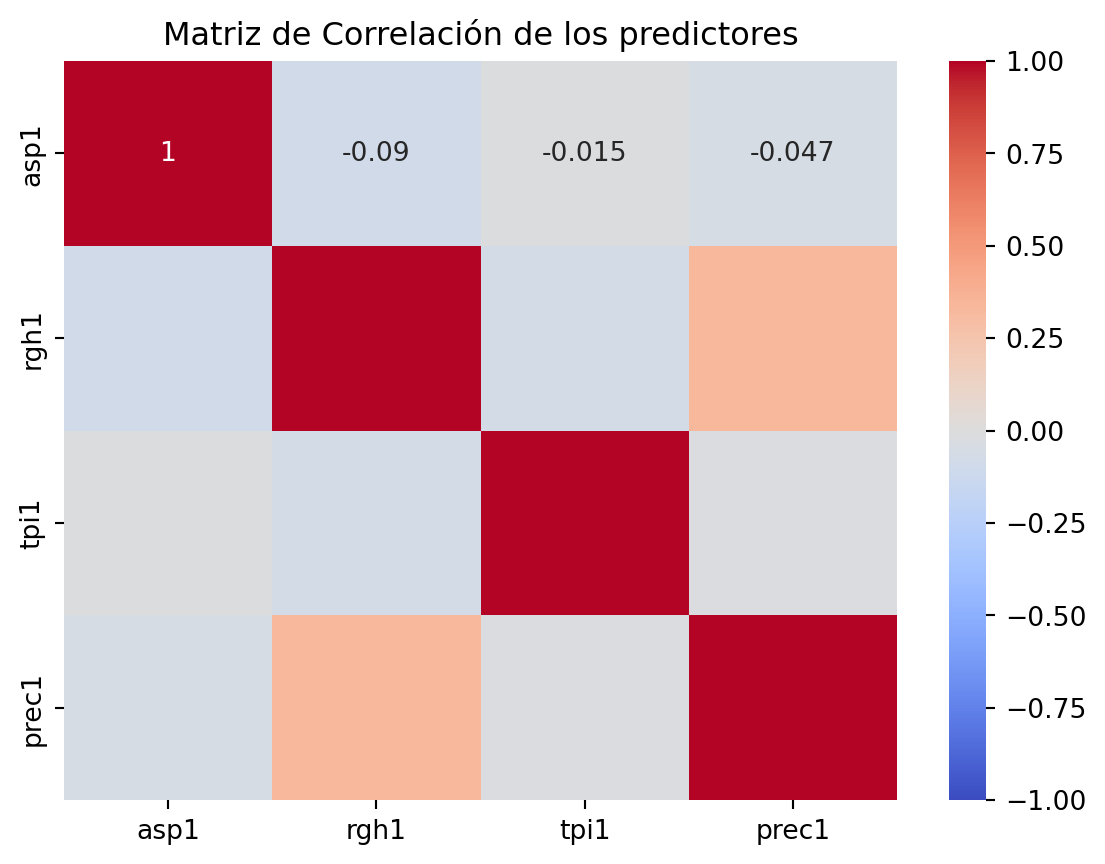
\includegraphics[keepaspectratio]{index_files/figure-pdf/cell-7-output-2.pdf}}

\subsection{2. División en conjuntos de entrenamiento y prueba
(train\_test\_split).}\label{divisiuxf3n-en-conjuntos-de-entrenamiento-y-prueba-train_test_split.}

Se dividen los datos: - 80\% para entrenar el modelo - 20\% para evaluar
su desempeño

\begin{Shaded}
\begin{Highlighting}[]
\NormalTok{X\_train, X\_test, y\_train, y\_test }\OperatorTok{=}\NormalTok{ train\_test\_split(}
\NormalTok{    X, y, test\_size}\OperatorTok{=}\FloatTok{0.3}\NormalTok{, random\_state}\OperatorTok{=}\DecValTok{42}
\NormalTok{)}

\BuiltInTok{print}\NormalTok{(}\StringTok{"Tamaño entrenamiento:"}\NormalTok{, X\_train.shape)}
\BuiltInTok{print}\NormalTok{(}\StringTok{"Tamaño prueba:"}\NormalTok{, X\_test.shape)}
\end{Highlighting}
\end{Shaded}

\begin{verbatim}
Tamaño entrenamiento: (8921, 4)
Tamaño prueba: (3824, 4)
\end{verbatim}

\subsection{3. Definición y entrenamiento del modelo utilizando
Pipeline.}\label{definiciuxf3n-y-entrenamiento-del-modelo-utilizando-pipeline.}

Etapas del pipeline:

\begin{itemize}
\tightlist
\item
  Imputer: reemplaza valores faltantes por la media.
\item
  Scaler: estandariza las variables (media = 0, desviación = 1).
\item
  Regresión logística: modelo lineal que estima la probabilidad de
  deslizamiento.
\item
  class\_weight=`balanced': ajusta el peso de las clases para evitar
  sesgo hacia la clase mayoritaria.
\end{itemize}

\begin{Shaded}
\begin{Highlighting}[]
\CommentTok{\# Definir pipeline: estandarización + regresión logística}
\CommentTok{\#pipe = Pipeline([}
\CommentTok{\#    (\textquotesingle{}imputer\textquotesingle{}, SimpleImputer(strategy=\textquotesingle{}mean\textquotesingle{})),  \# or \textquotesingle{}median\textquotesingle{}}
\CommentTok{\#    (\textquotesingle{}scaler\textquotesingle{}, StandardScaler()),}
\CommentTok{\#    (\textquotesingle{}logreg\textquotesingle{}, LogisticRegression(solver=\textquotesingle{}liblinear\textquotesingle{}, class\_weight=\textquotesingle{}balanced\textquotesingle{},max\_iter=1000))}
\CommentTok{\#])}

\NormalTok{pipe }\OperatorTok{=}\NormalTok{ Pipeline([}
\NormalTok{    (}\StringTok{\textquotesingle{}poly\textquotesingle{}}\NormalTok{, PolynomialFeatures(degree}\OperatorTok{=}\DecValTok{2}\NormalTok{, include\_bias}\OperatorTok{=}\VariableTok{False}\NormalTok{)),}
\NormalTok{    (}\StringTok{"scaler"}\NormalTok{, StandardScaler()),}
\NormalTok{    (}\StringTok{"regressor"}\NormalTok{, LinearRegression())}
\NormalTok{])}

\CommentTok{\# Entrenar modelo}
\NormalTok{pipe.fit(X\_train, y\_train)}
\end{Highlighting}
\end{Shaded}

\begin{verbatim}
Pipeline(steps=[('poly', PolynomialFeatures(include_bias=False)),
                ('scaler', StandardScaler()),
                ('regressor', LinearRegression())])
\end{verbatim}

\subsection{4. Generación de
predicciones.}\label{generaciuxf3n-de-predicciones.}

\begin{Shaded}
\begin{Highlighting}[]
\NormalTok{y\_pred }\OperatorTok{=}\NormalTok{ pipe.predict(X\_test)}
\NormalTok{y\_pred[:}\DecValTok{5}\NormalTok{]}
\CommentTok{\#y\_prob = pipe.predict\_proba(X\_test)[:, 1]}
\end{Highlighting}
\end{Shaded}

\begin{verbatim}
array([-0.04770735,  0.13927089,  0.21075155,  0.07770748, -0.09311675])
\end{verbatim}

\subsection{5. Evaluación del modelo con métricas
apropiadas.}\label{evaluaciuxf3n-del-modelo-con-muxe9tricas-apropiadas.}

\begin{Shaded}
\begin{Highlighting}[]
\NormalTok{mse }\OperatorTok{=}\NormalTok{ mean\_squared\_error(y\_test, y\_pred)}
\NormalTok{r2 }\OperatorTok{=}\NormalTok{ r2\_score(y\_test, y\_pred)}
\end{Highlighting}
\end{Shaded}

El \emph{Mean Squared Error (MSE)} mide cuánto se desvían en promedio
las predicciones de los valores reales. Un MSE de 0.22 significa que el
error cuadrático medio entre los valores reales del balance de masa y
los predichos por el modelo es aproximadamente 0.22 metros, siendo muy
alto y poco eficiente. Entonces el modelo no está logrando capturar bien
la relación entre las variables explicativas y la variable dependiente.

\begin{Shaded}
\begin{Highlighting}[]
\BuiltInTok{print}\NormalTok{(}\StringTok{"Mean Squared Error (MSE):"}\NormalTok{, mse)}
\end{Highlighting}
\end{Shaded}

\begin{verbatim}
Mean Squared Error (MSE): 0.22894841340348443
\end{verbatim}

El \emph{R²} mide la proporción de la variabilidad de la variable
objetivo que logra explicar el modelo. Un R² = 0.14 india que el modelo
solo explica aproximadamente el 14\% de la variación de los datos. Asi,
las variables explicativas actuales (aspecto, pendiente, elevación,
rugosidad, etc.) no son suficientes para explicar el comportamiento del
balance de masa.

\begin{Shaded}
\begin{Highlighting}[]
\BuiltInTok{print}\NormalTok{(}\StringTok{"R² Score:"}\NormalTok{, r2)}
\end{Highlighting}
\end{Shaded}

\begin{verbatim}
R² Score: 0.11863329007754908
\end{verbatim}

\subsection{6. Visualizaciones e interpretación de
resultados.}\label{visualizaciones-e-interpretaciuxf3n-de-resultados.}

En la matriz de comfusion Diagonal principal → predicciones correctas.
Fuera de la diagonal → errores del modelo.

\begin{Shaded}
\begin{Highlighting}[]
\ImportTok{import}\NormalTok{ matplotlib.pyplot }\ImportTok{as}\NormalTok{ plt}

\NormalTok{plt.figure(figsize}\OperatorTok{=}\NormalTok{(}\DecValTok{8}\NormalTok{,}\DecValTok{6}\NormalTok{))}
\NormalTok{plt.scatter(y\_test, y\_pred, alpha}\OperatorTok{=}\FloatTok{0.7}\NormalTok{)}
\NormalTok{plt.plot([y\_test.}\BuiltInTok{min}\NormalTok{(), y\_test.}\BuiltInTok{max}\NormalTok{()], [y\_test.}\BuiltInTok{min}\NormalTok{(), y\_test.}\BuiltInTok{max}\NormalTok{()], }\StringTok{\textquotesingle{}r{-}{-}\textquotesingle{}}\NormalTok{, lw}\OperatorTok{=}\DecValTok{2}\NormalTok{)}
\NormalTok{plt.xlabel(}\StringTok{"Valores Reales"}\NormalTok{)}
\NormalTok{plt.ylabel(}\StringTok{"Valores Predichos"}\NormalTok{)}
\NormalTok{plt.title(}\StringTok{"Regresión Lineal: Valores Reales vs Predichos"}\NormalTok{)}
\NormalTok{plt.show()}
\end{Highlighting}
\end{Shaded}

\pandocbounded{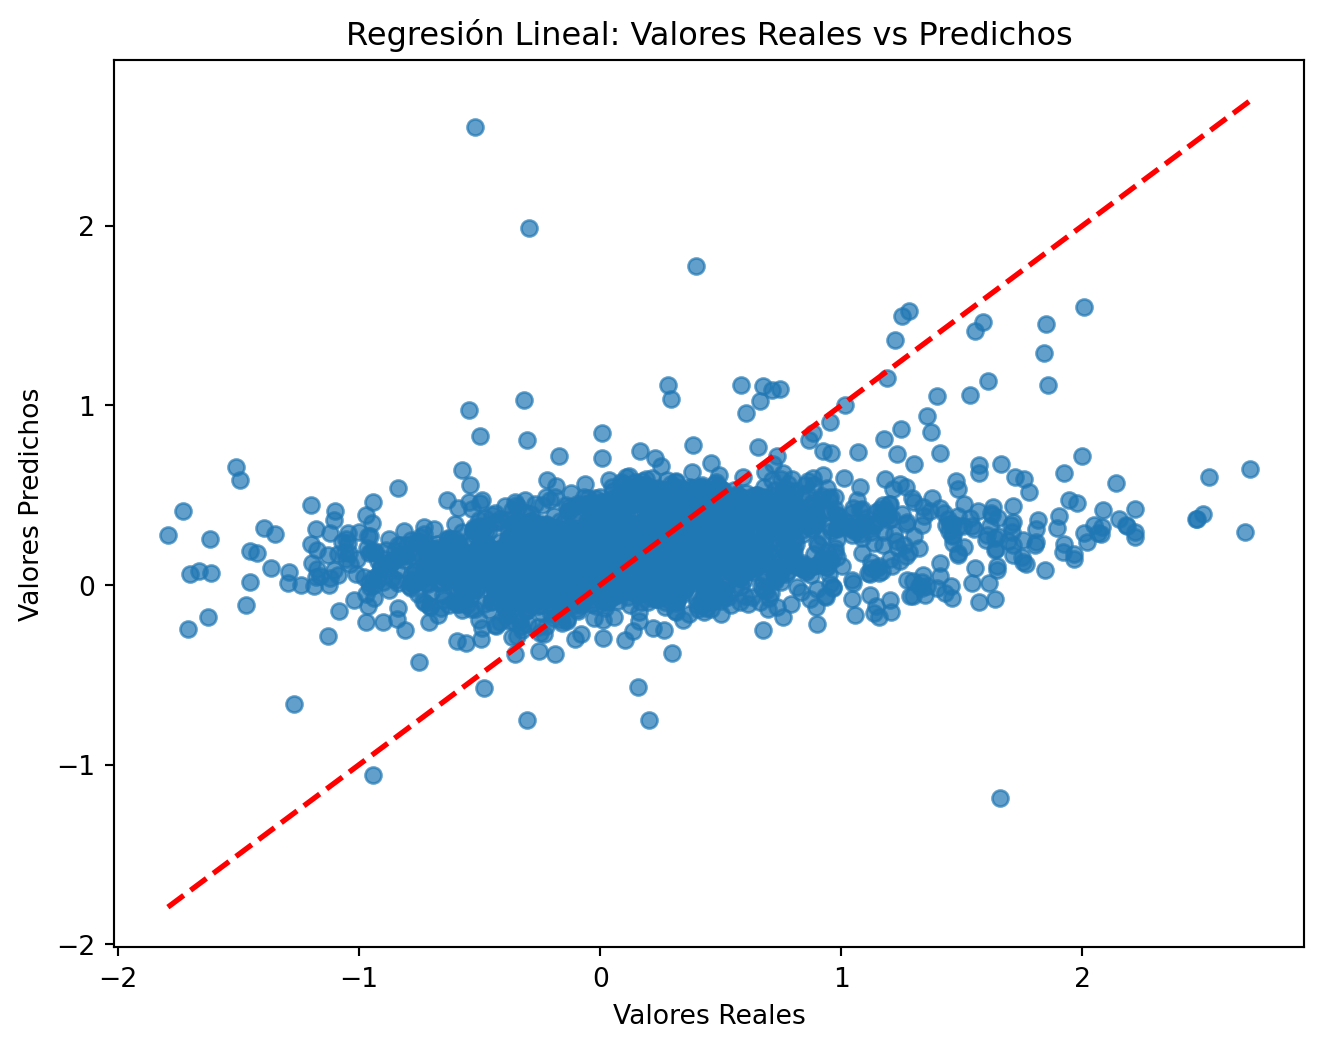
\includegraphics[keepaspectratio]{index_files/figure-pdf/cell-14-output-1.pdf}}




\end{document}
